\documentclass{article}

\usepackage{graphicx}
\usepackage{tikz}
\usepackage{tikzsymbols}
\usetikzlibrary{calc,patterns,shapes.geometric}
\pagestyle{empty}
\usepackage[margin=0pt]{geometry}
\geometry{papersize={14in,12in}}

\def\centerarc[#1](#2)(#3:#4:#5){\draw[#1] ($(#2)+({#5*cos(#3)},{#5*sin(#3)})$) arc (#3:#4:#5);}

\begin{document}
	\begin{figure}
		\centering
		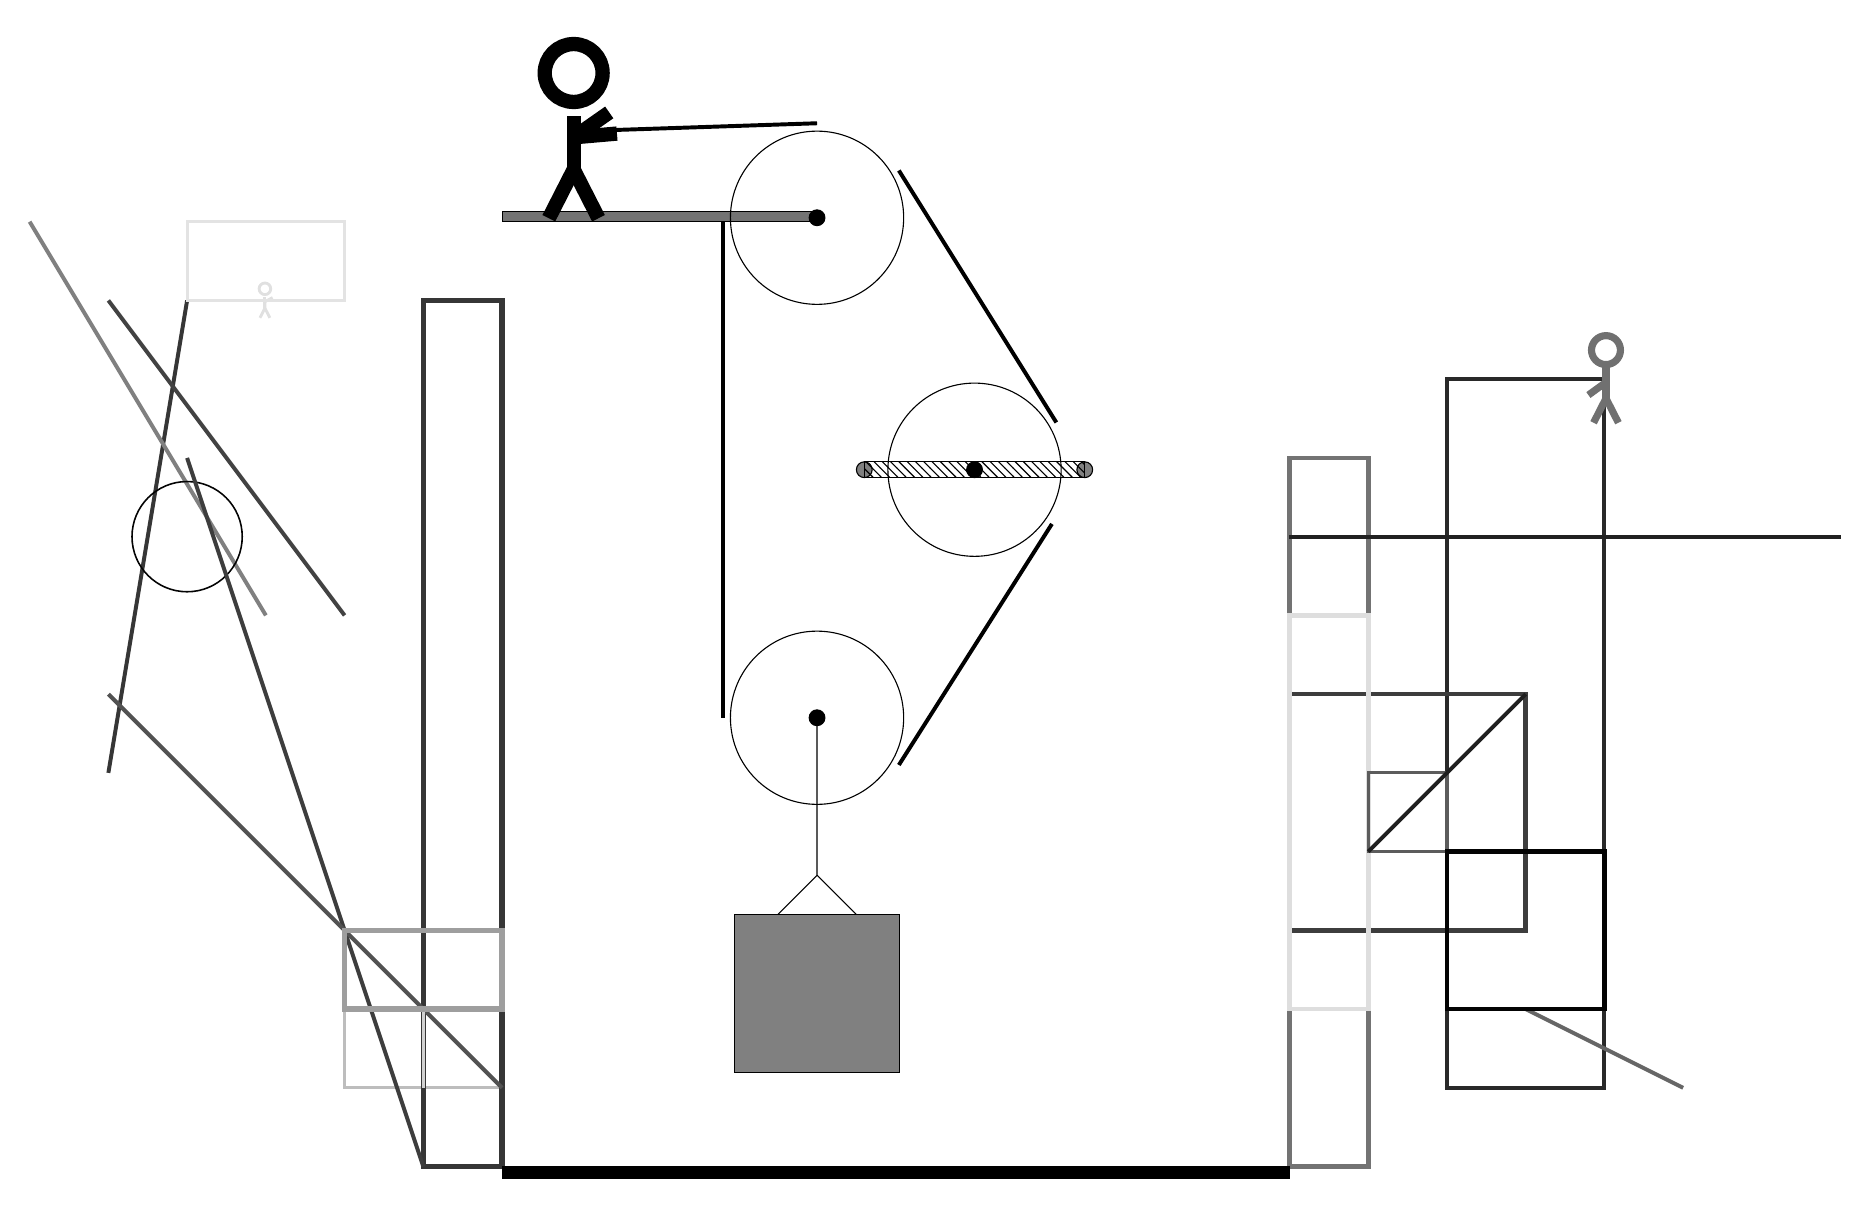
\begin{tikzpicture}
			%%%%% START %%%%%
			
			\draw[fill=black!55] (-2, 9) rectangle (2, 9.125);
			
			\draw (2, 2.7) circle (1.1);
			\draw[fill=black] (2, 2.7) circle (0.1);
			
			\draw (2, 9.05) circle (1.1);
			\draw[fill=black] (2, 9.05) circle (0.1);
			
			\draw[fill=white](4, 5.85) circle (1.1);
			\draw[fill=black] (4, 5.85) circle (0.1);
			\draw[fill=black!50] (2.6, 5.85) circle (0.1);
			\draw[fill=black!50] (5.4, 5.85) circle (0.1);
			\draw[pattern=north west lines, pattern color=black] (2.6, 5.95) rectangle (5.4, 5.75);
			
			\draw (2, 2.7) -- (2, 0.7) -- (1.5, 0.2) -- (2.5, 0.2) -- (2, 0.7);
			\draw[fill=black!50] (0.95, 0.2) rectangle (3.05, -1.8);
			
			\draw[line width=0.4mm, color=black!26] (-4, -1) rectangle (-2, -2);
			
			\node[line width=0.3mm, color=black!12] at (-5, 8) {\Strichmaxerl[2][89][28]};
			\draw[line width=0.5mm, color=black!79](-7, 2) -- (-6, 8);
			\draw[line width=0.5mm, color=black!50](-5, 4) -- (-8, 9);
			\draw[line width=0.7mm, color=black!79] (-2, -3) rectangle (-3, 8);
			\draw [line width=0.2mm, color=black!99](-6, 5) circle (0.7);
			\draw[line width=0.2mm, color=black!84] (10, -1) rectangle (10, 6);
			\draw[line width=0.5mm, color=black!84] (10, 7) rectangle (12, -2);
			\draw[line width=0.6mm, color=black!69] (9, 2) rectangle (9, -2);
			
			\draw[line width=0.6mm, color=black!55] (8, -3) rectangle (9, 6);
			
			\draw[line width=0.6mm, color=black!76] (8, 0) rectangle (11, 3);
			
			\draw[line width=0.5mm, color=black!76](-3, -3) -- (-6, 6);
			\draw[line width=0.5mm, color=black!68](-7, 3) -- (-2, -2);
			
			\draw[line width=0.4mm, color=black!11] (-4, 9) rectangle (-6, 8);
			\draw[line width=0.6mm, color=black!13] (9, 4) rectangle (8, -1);
			\draw[line width=0.5mm, color=black!74](-7, 8) -- (-4, 4);
			\draw[line width=0.5mm, color=black!87](8, 5) -- (15, 5);
			\draw[line width=0.4mm, color=black!64] (10, 2) rectangle (9, 1);
			\node[line width=0.6mm, color=black!56] at (12, 7) {\Strichmaxerl[5][36][90]};
			\draw[line width=0.3mm, color=black!18] (-3, -2) rectangle (-3, -1);
			\draw[line width=0.5mm, color=black!88](9, 1) -- (11, 3);
			
			\draw[line width=0.7mm, color=black!38] (-2, -1) rectangle (-4, 0);
			\draw[line width=0.5mm, color=black!60](11, -1) -- (13, -2);
			\draw[line width=0.6mm, color=black!99] (10, -1) rectangle (12, 1);
			
			\draw[line width=0.5mm] (0.8, 9) -- (0.8, 2.7);
			\centerarc[line width=0.5mm](2, 2.7)(180:330:1.2000000000000002);
			\draw[line width=0.5mm](3.0392, 2.1) -- (4.983, 5.1617);
			\centerarc[line width=0.5mm](4, 5.85)(390:325:1.2000000000000002);
			\draw[line width=0.5mm](5.0392, 6.45) -- (3.0392, 9.65);
			\centerarc[line width=0.5mm](2, 9.05)(30:90:1.2000000000000002);
			\draw[line width=0.5mm](2, 10.25) -- (-1, 10.15);
			
			\node at (-1, 10.15) {\Strichmaxerl[10][-175][35]};
			
			\draw[fill=black] (-2, -3) rectangle (8, -3.15);
			
			%%%%% END %%%%%
		\end{tikzpicture}
	\end{figure}	
\end{document}